\documentclass[10.5pt, a4paper]{article}
\usepackage[paperheight=32cm,paperwidth=21cm,includehead,nomarginpar,textwidth=18cm,textheight=27cm,headheight=4mm]{geometry}
\usepackage{fancyhdr}
\usepackage[utf8]{vietnam}
\usepackage[english]{babel}
\usepackage{xcolor,amsmath,amssymb,amsfonts}
\usepackage[most]{tcolorbox}
\usepackage{graphicx}
\title{\color{red}\textbf{Đề tài giữa học kì I Lý thuyết độ đo và tích phân}}
\author{\color{red}Lê Hoàng Bảo - MSSV: 21110040}
\date{\color{red}07 tháng 12 năm 2023}
\begin{document}
% Set the page style to "fancy"...
\pagestyle{fancy}
%... then configure it.
\fancyhead{} % clear all header fields
\fancyhead[R]{\textbf{Trường Đại học Khoa học Tự nhiên, ĐHQG-HCM\\Bộ môn Giải tích, Khoa Toán - Tin học}}
\fancyhead[L]{\color{red}\textbf{\LaTeX~by Lê Hoàng Bảo}}
\fancyfoot{} % clear all footer fields
\fancyfoot[R]{Mã môn học: MTH10462}
\fancyfoot[L]{LÝ THUYẾT ĐỘ ĐO}
\fancyfoot[C]{\textbf\thepage}
\renewcommand{\headrulewidth}{0.7pt}
\renewcommand{\footrulewidth}{0.7pt}
\maketitle
\begin{center}
    Giảng viên: PGS.TS. Bùi Lê Trọng Thanh
\end{center}
\begin{center}
    \textbf{Nội dung đề tài: CANTOR TERNARY SET AND CANTOR-LEBESGUE FUNCTION}
\end{center}
\newpage
\section{Tập Cantor}
\vspace{2mm}
Tập Cantor là một tập con khá lý thú của đoạn đóng $[0,1]$ với nhiều tính chất giúp chúng ta hình dung được những nội dung trong Giải tích. Nó có thể đóng vai trò như là các phản ví dụ hoặc edge-cases để kiểm chứng các ý tưởng trên chúng, và để xây dựng những thứ không thường thấy; một trong số đó là hàm Cantor mà ta sẽ làm rõ về nó trong đề tài này. Như chúng ta sẽ thấy trong bài này, tập Cantor không trù mật, nhưng lại không đếm được.
\subsection{Cách xây dựng}
\vspace{1mm}
Ta sẽ định nghĩa một họ tập hợp $\{E_n\}_{n=0}^\infty\subseteq[0,1]$, và định nghĩa tập Cantor là $K:=\displaystyle\bigcap_{n=0}^\infty E_n$.\\\\
Để bắt đầu, ta đặt: $$E_0=[0,1]$$
Chia đoạn $E_0$ thành ba đoạn bằng nhau, sau đó bỏ đi phần ở giữa, ta được: $$E_1=\left[0,\dfrac13\right]\cup\left[\dfrac23,1\right]$$
Lặp lại chu trình này bằng cách bỏ phần ở giữa của từng đoạn nhỏ trong $E_1$, ta được: $$E_2=\left[0,\dfrac19\right]\cup\left[\dfrac29,\dfrac39\right]\cup\left[\dfrac69,\dfrac79\right]\cup\left[\dfrac89,1\right]$$
Một cách tổng quát, ta định nghĩa $E_n$ theo $E_{n-1}$ bằng cách bỏ đi phần chính giữa của các đoạn tạo thành $E_{n-1}$. Ta có thể viết định nghĩa này như sau: $$E_n=\dfrac{E_{n-1}}{3}\cup\left(\dfrac23+\dfrac{E_{n-1}}{3}\right),~~~E_0=[0,1]$$
Hình dưới đây miêu tả tập Cantor, với thứ tự từ trên xuống lần lượt là $E_0$ đến $E_4$.
\begin{center}
    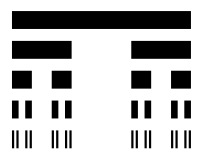
\includegraphics[width=0.4\linewidth]{cantor.png}
\end{center}
Với cách này, ta đã xây dựng một dãy tập hợp giảm: $E_0\supset E_1\supset\ldots\supset E_n\supset\ldots$\\\\
\underline{Nhận xét:} Qua cách xây dựng, ta có $E_n$ là hội của $2^n$ đoạn đóng rời nhau, với mỗi đoạn có chiều dài là $3^{-n}$. Đây chính là chìa khóa mà ta sẽ sử dụng để chứng minh các tính chất của tập Cantor.
\subsection{Các tính chất}
\vspace{1mm}
Cho $K:=\displaystyle\bigcap_{n=0}^\infty E_n$. Ta có các tính chất sau:\\\\
(i) $K$ là tập đóng.\\\\
(ii) Phần trong của $K$ là tập rỗng, hay $\mathring K=\varnothing$\\\\
(iii) $K$ không có điểm cô lập\\\\
(iv) $x\in K\Longleftrightarrow x=\displaystyle\sum_{k=1}^\infty\dfrac{a_k}{3^k}$ với $(a_k)$ là một dãy các số thực chỉ gồm hai số 0 và 2.\\\\
(v) $K$ không đếm được.
\newpage
\textbf{Chú ý:} Một tập được gọi là không trù mật nếu bao đóng của nó có phần trong rỗng. Do đó (i) và (ii) chỉ ra rằng $K$ không là tập trù mật.\\\\
\underline{\textit{Chứng minh:}}\\\\
(i) $E_n$ là tập đóng với mỗi $n$ nên $K=\displaystyle\bigcap_{n=0}^\infty E_n$ cũng là tập đóng. $\square$\\\\
(ii) Giả sử $\mathring K\ne\varnothing$, khi đó $\exists x\in\mathring K$. Do đó, với hữu hạn $\delta>0$ thì: $$B(x,\delta)\subseteq\mathring K\subseteq K$$
Chọn $n\in\mathbb N$ đủ lớn sao cho $3^{-n}<2\delta$. Ta có: $$(x-\delta,~x+\delta)\subseteq K\subseteq E_n$$
Tuy nhiên $E_n$ là hội rời của các đoạn có độ dài $3^{-n}<2\delta$, mâu thuẫn với điều giả sử. $\square$\\\\
(iii) Điểm mút cuối của các đoạn trong $E_n$ không bị bỏ đi trong các tập con $E_m$ với $m>n$. Tất cả điểm mút cuối $\left\{0,1,\frac13,\frac23,\dots\right\}\subset K$.\\\\
Cho trước $x\in K$ và $\varepsilon>0$. Ta chọn $n$ đủ lớn sao cho $3^{-n}<\varepsilon$. Khi đó $x\in E_n\Longrightarrow x\in[a,b]$ với $[a,b]\subset E_n$, một trong số $2^n$ đoạn đóng tạo thành $E_n$. Vì mỗi đoạn nhỏ có độ dài $3^{-n}$ nên $b-a<\varepsilon$, dẫn đến: $$|x-b|<\varepsilon,~~~~~~|x-a|<\varepsilon$$
Vì vậy, kể cả khi $x=a$ hay $x=b$, ta đã tìm được $y\ne x$ sao cho $y\in K\cap B(x,\varepsilon)~\square$\\\\
(iv) Xét $\frac13\in K$, khi đó $\frac13=\sum_{k=1}^\infty\frac{a_k}{3}$. Ta có thể thu được một mở rộng bậc ba với $a_1=1$ và $a_n=0$ với $n>1$, nhưng không thỏa điều kiện được đặt ra. Nhưng ta có thể chọn các hệ số khác: $$\displaystyle\sum_{k=1}^\infty\dfrac{2}{3^k}=2\cdot\dfrac19\displaystyle\sum_{k=0}^\infty\left(\dfrac13\right)^k=\dfrac29\cdot\dfrac{1}{1-\frac13}=\dfrac13$$
Nói cách khác, các mở rộng bậc ba không là duy nhất. Tuy nhiên, các mở rộng bậc ba mà chỉ chứa các số 0 hoặc 2 là \textit{duy nhất}. Đó là nội dung của các hệ quả sau:\\\\
$\bullet~$\textbf{Hệ quả 1:} Nếu: $$\displaystyle\sum_{k=1}^\infty\dfrac{a_k}{3^k}=\displaystyle\sum_{k=1}^\infty\dfrac{b_k}{3^k}$$ với mỗi $a_k,b_k\in\{0,2\}$ thì $a_k=b_k$ với mọi $k\in\mathbb N$\\\\
\underline{\textit{Chứng minh:}} Ta giả sử điều ngược lại, thì sẽ tồn tại $N$ nhỏ nhất sao cho $a_n\ne b_n$, lúc đó một trong hai giá trị $a_n$ hoặc $b_n$ sẽ bằng 0. Khai triển tổng: $$\displaystyle\sum_{k=1}^{N-1}\dfrac{a_k}{3^k}+0+\displaystyle\sum_{k=N+1}^\infty\dfrac{a_k}{3^k}=\displaystyle\sum_{k=1}^{N-1}\dfrac{b_k}{3^k}+\dfrac{2}{3^N}+\displaystyle\sum_{k=N+1}^\infty\dfrac{b_k}{3^k}$$
Sử dụng dữ liệu $a_k=b_k$ với $k<N$: $$\displaystyle\sum_{k=N+1}^\infty\dfrac{a_k}{3^k}=\dfrac{2}{3^N}+\displaystyle\sum_{k=N+1}^\infty\dfrac{b_k}{3^k}~~~~(*)$$
Nhưng: $$\displaystyle\sum_{k=N+1}^\infty\dfrac{a_k}{3^k}\le2\displaystyle\sum_{k=N+1}^\infty3^{-k}=2.3^{-N-1}\displaystyle\sum_{k=0}^\infty3^{-k}=2.3^{-N-1}\cdot\dfrac{1}{1-\frac13}=3^{-N}$$
Vậy, quay trở lại $(*)$, ta có: $$\dfrac{2}{3^N}+\displaystyle\sum_{k=N+1}^\infty\dfrac{b_k}{3^k}\le\dfrac{1}{3^N}\Longrightarrow\displaystyle\sum_{k=N+1}^\infty\dfrac{b_k}{3^k}\le-\dfrac{1}{3^N}$$
hiển nhiên mâu thuẫn do $b_k=\{0,2\}$\\\\
$*$ Giờ ta đặt $S=\left\{\displaystyle\sum_{k=1}^\infty\dfrac{a_k}{3^k}:a_k\in\{0,2\}\right\}$. Nếu $x\in S$ thì $x=\displaystyle\sum_{k=1}^\infty\dfrac{a_k}{3^k}$ với hữu hạn $a_k\in\{0,2\}$.\\\\
Ta gọi $x_n=\displaystyle\sum_{k=1}^n\dfrac{a_k}{3^k}$ là tổng riêng phần thứ $n$.
\newpage
$\bullet~$\textbf{Hệ quả 2:} Với mỗi $n$, tổng riêng phần $x_n$ là điểm mút đầu của các đoạn đóng trong $E_n$.\\\\
\underline{\textit{Chứng minh:}} Bằng phương pháp quy nạp theo $n$: $x_1$ hoặc bằng 0 hoặc bằng $\frac23$, một trong hai giá trị sẽ là điểm mút đầu của $E_1$. Giả sử $x_{n-1}$ là điểm mút đầu của $E_{n-1}$, khi đó: $$\left[x_{n-1},~x_{n-1}+\dfrac{1}{3^{n-1}}\right]\subset E_{n-1}$$
Bằng sự xây dựng của $E_n$, ta có thể bỏ đi phần chính giữa để có được các đoạn đóng của $E_n$ như sau: $$\left[x_{n-1},~x_{n-1}+\dfrac{1}{3^n}\right]\cup\left[x_{n-1}+\dfrac{2}{3^n},~x_{n-1}+\dfrac{1}{3^{n-1}}\right]\subset E_n$$
Vậy nên $x_n=x_{n-1}+\dfrac{a_n}{3^n}$ là điểm mút đầu của một đoạn trong $E_n$, nếu $a_n=0$ hoặc $a_n=2.~\square$\\\\
Vì mỗi $x_n$ là một điểm mút đầu của $E_n$ và ta không bỏ điểm mút, ta có $x_n\in K$ với mọi $n$. Tuy nhiên $K$ là tập đóng nên chứa tất cả các điểm tụ, và ta có: $x:=\displaystyle\lim_{n\rightarrow\infty}x_n\in K$. Do đó $S\subset K$.\\\\
Để chỉ ra rằng $K\subset S$, ta chứng minh phản đảo đề: $x\notin S\Longrightarrow x\notin K$. Trước hết, ta chú ý thuộc tính sau.\\\\
$\bullet~$\textbf{Hệ quả 3:} Các khoảng bị bỏ đi để tạo thành $K$ đều có dạng: $$I_{k,m}=\left(\dfrac{3k+1}{3^m},\dfrac{3k+2}{3^m}\right):m\in\mathbb N,~~~0\le k\le3^{m-1}-1$$
hoặc nói cách khác: $$[0,1]\backslash E_n=\displaystyle\bigcup_{m=1}^n\displaystyle\bigcup_{k=0}^{3^{m-1}-1}I_{k,m}$$\\\\
Ta tiến tới việc chứng minh phản đảo đề. Giả sử $x\notin S$, và $x$ chứa số "1" trong chứ số thứ $n$ của khai triển bậc ba của nó: $$x=\displaystyle\sum_{k=1}^{n-1}\dfrac{a_k}{3^k}+\dfrac{1}{3^n}+\displaystyle\sum_{k=n+1}^\infty\dfrac{a_k}{3^k}$$
Ta sẽ lấy $n$ như là chữ số đầu tiên, là "1", nếu có nhiều hơn một chữ số.\\\\
$\bullet~$\textbf{Hệ quả 4:} Ta có $0<\displaystyle\sum_{k=n+1}^\infty\dfrac{a_k}{3^k}<\dfrac{1}{3^n}$\\\\
\underline{\textit{Chứng minh:}} Nếu $a_k=0$ với mọi $k>n$, thì số đó dưới dạng khải triển bậc ba sẽ có dạng $x=0,*1000\ldots$ với $*$ đại diện cho $n-1$ chữ số đầu tiên thuộc $\{0,2\}$. Thay vào đó ta có thể chọn $x=0,*2222\ldots$, tránh chữ số 1. Nói cách khác, $x\in S$. Tương tự, nếu $a_k=2$ với mọi $k>n$ thì ta viết $x=0,*1222\ldots$, vậy $x$ thừa nhận mở rộng $x=0,*2222\ldots$, và do đó $x\in S$. Vì thế nếu $x\notin S$ thì điều kiện trên vẫn đúng. $\square$\\\\
Giờ ta có thể viết lại: $$\displaystyle\sum_{k=1}^{n-1}\dfrac{a_k}{3^k}=\displaystyle\sum_{k=1}^{n-1}\dfrac{3(3^{n-k-1}a_k)}{3^k}=\dfrac{3\lambda}{3^k}$$
với $\lambda=\displaystyle\sum_{k=1}^{n-1}3^{n-k-1}a_k\in\mathbb N\cup\{0\}$. Với định nghĩa này, thì Hệ quả 4 cho ta: $$\dfrac{3\lambda+1}{3^n}<x<\dfrac{3\lambda+2}{3^n}$$
Vậy $x\in I_{\lambda,n}$ và do đó $x\notin K$ theo Hệ quả 3.\\\\
(v) $K$ không đếm được, tức $|K|=|[0,1]|$. Ta đã biết rằng $K\subset[0,1]$, do đó $|K|\le|[0,1]|$. Vì thế nên ta cần tìm một toàn ánh từ $K\rightarrow[0,1]$ để hoàn thành việc chứng minh.\\\\
Ta định nghĩa một ánh xạ $F:K\rightarrow[0,1]$ sao cho $F$ lấy $x\in K$ và đổi tất cả các chữ số "2" trong khai triển bậc ba của nó thành "1", sau đó xuất ra giá trị với khai triển nhị phân tương ứng. Ta có: $$K=\left\{\displaystyle\sum_{k=1}^\infty\dfrac{a_k}{3^k}:a_k\in\{0,2\}\right\}$$
Với $x\in K$, ta viết $x=\displaystyle\sum_{k=1}^\infty\dfrac{a_k}{3^k}$ với $a_k\in\{0,2\}$. Sau đó ta định nghĩa: $$F(x)=\displaystyle\sum_{k=1}^\infty\dfrac{a_k}{2}\dfrac{1}{2^k}$$
Vì Bổ đề 1, ta có khai triện bậc ba duy nhất của $x$ mà không chứa "2", và ta có được hàm định nghĩa tốt.\\\\
Cho $y\in[0,1]$, thì $y$ thừa nhận một khai triển nhị phân: $y=\sum_{k=1}^\infty\frac{b_k}{2^k}$ với $b_k\in\{0,1\}$. Khi đó đặt $x=\sum_{k=1}^\infty\frac{2b_k}{3^k}$ sao cho $F(x)=\sum_{k=1}^\infty\frac{b_k}{2^k}=y$. Vậy ta đã hoàn thành việc chứng minh. $\square$
\section{Hàm Cantor - Lebesgue}
Một tập mở $G$ mà được định nghĩa trong sự xây dựng của tập Cantor là hội rời của các tập mở: $$I_{1,1},I_{2,1},I_{2,2},I_{3,1},I_{3,2},\dots,I_{k,1},\dots,I_{k,2^{k-1}},\dots$$
với $|I_{k,j}|=\dfrac{1}{3^k},~j=\overline{1,\dots,2^{k-1}},~k\in\mathbb N$. Ta tiến hành định nghĩa một hàm thực $\tau_0$ trên $G$: $$\tau_0(x)=\begin{cases}
    \frac12,~~~~~~~~~~~~~~~~~x\in I_{1,1}\\
    \frac{1}{2^2},\frac{3}{2^2},~~~~~~~~~~~x\text{ lần lượt thuộc }I_{2,1},I_{2,2}\\
    \frac{1}{2^3},\frac{3}{2^3},\frac{5}{2^3},\frac{7}{2^3},~~x\text{ lần lượt thuộc }I_{3,1},I_{3,2},I_{3,3},I_{3,4}\\
    \vdots\\
    \frac{1}{2^k},\dots,\frac{2^k-1}{2^k},~~x\text{ lần lượt thuộc }I_{k,1},\dots,I_{k,2^{k-1}}\\
    \vdots
\end{cases}$$
Ta thấy $\tau_0$ là hàm tăng trên $G$. Nếu $x'$ và $x''$ là hai điểm trong $G$, và nếu khoảng cách giữa chúng nhỏ hơn $\frac{1}{3^k}$, thì khoảng cách giữa $\tau_0(x')$ và $\tau_0(x'')$ không vượt quá $\frac{1}{2^k}$. Do đó với mọi $\varepsilon>0$, nếu $k\in\mathbb N$ lớn đến độ $\frac{1}{2^k}<\varepsilon$ thì: $$x',x''\in G,~|x'-x''|<\dfrac{1}{3^k}\Rightarrow|\tau_0(x')-\tau_0(x'')|\le\dfrac{1}{2^k}<\varepsilon$$
Vì vậy $\tau_0$ \textit{liên tục đều} trên $G$. Điều này nói rằng $\tau_0$ có một khai triển liên tục duy nhất tới $\overline G$. Vì $G$ trù mật trong $[0,1]$ nên ta có $\overline G=[0,1]$. Đặt $\tau$ là một khai triển liên tục của $\tau_0$ tới $[0,1]$. Ta gọi hàm này là hàm Cantor - Lebesgue trên $[0,1]$.\\\\
$\bullet~$\textbf{Định lý:} Hàm Cantor - Lebesgue $\tau$ trên $[0,1]$ có các tính chất sau:\\\\
(i) $\tau$ liên tục trên $[0,1]$.\\\\
(ii) $\tau$ tăng trên $[0,1]$.\\\\
(iii) $\tau(0)=0$ và $\tau(1)=1$.\\\\
\underline{Chứng minh:} Theo định nghĩa thì $\tau$ liên tục trên $[0,1]$. Để chứng minh $\tau$ tăng trên $[0,1]$, đặt $x',x''\in[0,1]$ và $x'<x''$. Vì $G$ trù mật trong $[0,1]$, ta có thể chọn hai dãy $(a_n)_{n\in\mathbb N}$ và $(b_n)_{n\in\mathbb N}$ trong $G$ sao cho $a_n<b_n$ với mọi $n\in\mathbb N$ và $a_n\rightarrow x'^+,~b_n\rightarrow x''^-$. Vì sự liên tục của $\tau$ trên $[0,1]$, ta có $\displaystyle\lim_{n\rightarrow\infty}\tau(a_n)=\tau(x')$ và $\displaystyle\lim_{n\rightarrow\infty}\tau(b_n)=\tau(x'')$. Vì $\tau$ tăng trên $G$ và $a_n,b_n\in G$ với $a_n<b_n$, ta có $\tau(a_n)\le\tau(b_n)$ với $n\in\mathbb N$. Do đó $\displaystyle\lim_{n\rightarrow\infty}\tau(a_n)\le\displaystyle\lim_{n\rightarrow\infty}\tau(b_n)$, tức là $\tau(x')\le\tau(x'')$. Vậy $\tau$ tăng trên $[0,1]$.\\\\
Để chứng minh $\tau(0)=0$, xét một dãy các khoảng trong sự xây dựng của $T:$ $$I_{1,1}=\left(\dfrac13,\dfrac23\right),~I_{2,1}=\left(\dfrac{1}{3^2},\dfrac{2}{3^2}\right),~I_{3,1}=\left(\dfrac{1}{3^3},\dfrac{2}{3^3}\right),\ldots,I_{k,1}=\left(\dfrac{1}{3^k},\dfrac{2}{3^k}\right),\ldots$$
Cho $x_k=\frac32\frac{1}{3^k}$ là trung điểm của $I_{k,1}$ với $k\in\mathbb N$, khi đó $\displaystyle\lim_{k\rightarrow\infty}x_k=0$. Từ định nghĩa của $\tau$ trên $G$, ta có $\tau(x_k)=\frac{1}{2^k}$. Khi đó, bởi sự liên tục của $\tau$ tại $x=0$, ta có: $$\tau(0)=\tau\left(\displaystyle\lim_{k\rightarrow\infty}x_k\right)=\displaystyle\lim_{k\rightarrow\infty}\tau(x_k)=\displaystyle\lim_{k\rightarrow\infty}\dfrac{1}{2^k}=0$$
Lập luận tương tự, ta cũng có $\tau(1)=1.~\square$\\\\
$\bullet~$\textbf{Bổ đề:} Cho $\varphi=\tau+i$ với $\tau$ là hàm Cantor - Lebesgue trên $[0,1]$ và $i$ là một ánh xạ đồng nhất trên $[0,1]$, tức là $i(x)=x,~\forall x\in[0,1]$. Khi đó $\varphi$ là một phép đồng phôi của $[0,1]$ lên $[0,2]$. Hơn nữa $\varphi$ và hàm ngược của nó là $\psi$ là hai hàm tăng ngặt trên miền xác định tương ứng của chúng.\\\\
\underline{Chứng minh:} Vì $\tau$ và $i$ đều là hai hàm thực liên tục và tăng trên $[0,1]$ nên $\varphi=\tau+i$ cũng thế. Vì $\tau(0)=0,\tau(1)=1,i(0)=0$ và $i(1)=1$ nên ta có $\varphi(0)=0$ và $\varphi(1)=2$. Theo Định lý giá trị trung bình của hàm liên tục, với mọi $\alpha\in(0,2)$ thì tồn tại $x\in(0,1)$ sao cho $\varphi(x)=\alpha$. Do đó $\varphi([0,1])=[0,2]$.\\\\
Trên $[0,1]$, vì $\tau$ là hàm tăng và $i$ là hàm tăng ngặt nên $\varphi=\tau+i$ cũng tăng ngặt trên $[0,1]$, và vì thế $\varphi$ là một song ánh đi từ $[0,1]$ đến $[0,2]$, dẫn đến $\varphi$ là một phép đồng phôi của $[0,1]$ lên $[0,2]$. Hàm ngược $\psi$ của $\varphi$ được xác định trên $[0,2]$ và là một song ánh đi từ $[0,2]$ đến $[0,1]$. Vì $\varphi$ là hàm tăng trên $[0,1]$ nên $\psi$ tăng trên $[0,2]$. Do $\psi$ là một song ánh, nên nó tăng ngặt. $\square$\\\\
$\bullet~$\textbf{Mệnh đề:} Tồn tại một hàm $f$ tăng ngặt, liên tục trên $[0,1]$ và một tập compact $K\subset[0,1]$ sao cho $K$ là tập rỗng trong $(\mathbb R,\mathcal B_{\mathbb R},\mu_L)$ và $\mu_L(f(K))=1$.\\\\
\underline{Chứng minh:} Ta sẽ chứng minh hàm $\varphi=\tau+i$ ở bổ đề trên và tập Cantor $T$ là hàm $f$ và tập $K$ tương ứng.\\\\
Cho $G$ là tập mở được định nghĩa dựa trên sự xây dựng của $T.~G$ là hội đếm được của các khoảng mở rời nhau. Đặt $(J_n)_{n\in\mathbb N}$ là một họ các khoảng mở xây dựng nên $G$. Cho $c_n$ là giá trị của hàm Cantor - Lebesgue trên $J_n$, khi đó $\varphi(J_n)=(\tau+i)(J_n)=J_n+c_n$. Do đó: $$\varphi(G)=\varphi\left(\displaystyle\bigcup_{n\in\mathbb N}J_n\right)=\displaystyle\bigcup_{n\in\mathbb N}(J_n+c_n)\in\mathcal B_{\mathbb R}$$
Với $m\ne n$, nếu khoảng mở $J_n$ nằm phía bên trái khoảng mở $J_m$ thì $c_n<c_m$ vì $\tau$ là hàm tăng. Do đó $J_n+c_n$ và $J_m+c_m$ rời nhau. Khi đó, với tính cộng tính đếm được của $\mu_L$, và với sự dịch chuyển bất biến của $(\mathbb R,\mathfrak M_L,\mu_L)$ thì: $$\mu_L(\varphi(G))=\displaystyle\sum_{n\in\mathbb N}\mu_L(J_n+c_n)=\displaystyle\sum_{n\in\mathbb N}\mu_L(J_n)=\mu_L(G)=1$$
Giờ ta có: $$\varphi(T)=\varphi([0,1]\backslash G)=\varphi([0,1])\backslash\varphi(G)=[0,2]\backslash\varphi(G)\in\mathcal B_{\mathbb R}$$
nên $\mu_L(\varphi(T))=\mu_L([0,2])-\mu_L(\varphi(G))=2-1=1$. Do đó với tập Cantor $T$ (là tập compact trên $\mathbb R$ và là tập rỗng trên $(\mathbb R,\mathcal B_{\mathbb R},\mu_L)$) và với hàm liên tục tăng ngặt $\varphi$ trên $[0,1]$, ta có $\mu_L(\varphi(T))=1$. $\square$
\end{document}